\emergencystretch=3em
\subsection{Datos y método de análisis}

El análisis usa únicamente los CSV de la campaña oficial (carpeta \path|campana-oficial-20261121-223100| dentro de \path|data/|), cuyas sumas SHA-256 se comprobaron con \path|SHA256SUMS|. Por cada mecanismo hay 2\,400 filas de latencia: 100 envíos por corrida, seis corridas (un calentamiento y cinco registradas) en cada combinación de tamaño (100 y 10\,240 bytes) y modo (secuencial y concurrente). El calentamiento se excluye del análisis; no hubo fallos en ninguna corrida registrada. Las pruebas se ejecutaron el 21 de noviembre de 2026 con los tres nodos como procesos en \texttt{localhost}, en un equipo con Windows 11, procesador AMD64 de 16 GB de RAM y Python 3.12.7 (\path|entorno.md|).

El script \path|analysis/analizar.py| calcula, por mecanismo, tamaño y modo: media, mediana, desviación estándar, percentil 95 y un intervalo de confianza del 95\,\% de la media obtenido por \emph{bootstrap} con semilla fija. El rendimiento es el total de solicitudes completadas dividido por la duración de pared de las corridas registradas. La tabla y los gráficos de esta sección los genera el mismo script, de modo que no hay cifras escritas a mano.

\subsection{Latencia y rendimiento}

\begin{table}[htbp]
\centering
\footnotesize
\setlength{\tabcolsep}{3pt}
\caption{Latencia y rendimiento por mecanismo, tamaño y modo (calentamiento excluido)}
\label{tab:resumen-latencia}
\begin{tabular}{@{}llrrrrrrr@{}}
\toprule
\textbf{Modo} & \textbf{Mecanismo} & \textbf{Bytes} & \textbf{n} & \textbf{Media} & \textbf{Med.} & \textbf{Desv.} & \textbf{p95} & \textbf{Msg/s} \\
\midrule
concurrente & gRPC & 100 & 500 & 0.559 & 0.542 & 0.092 & 0.751 & 3814 \\
concurrente & Sockets TCP & 100 & 500 & 0.198 & 0.177 & 0.088 & 0.298 & 6047 \\
concurrente & gRPC & 10240 & 500 & 0.827 & 0.756 & 0.299 & 1.340 & 2373 \\
concurrente & Sockets TCP & 10240 & 500 & 0.282 & 0.263 & 0.084 & 0.415 & 4469 \\
secuencial & gRPC & 100 & 500 & 0.644 & 0.484 & 0.311 & 1.206 & 1199 \\
secuencial & Sockets TCP & 100 & 500 & 0.150 & 0.139 & 0.047 & 0.213 & 3409 \\
secuencial & gRPC & 10240 & 500 & 0.528 & 0.515 & 0.088 & 0.688 & 1342 \\
secuencial & Sockets TCP & 10240 & 500 & 0.320 & 0.308 & 0.116 & 0.472 & 1486 \\
\bottomrule
\end{tabular}
\par\smallskip\footnotesize Latencias en milisegundos. n = envíos válidos de cinco corridas registradas por combinación.
\end{table}


\begin{figure}[htbp]
\centering
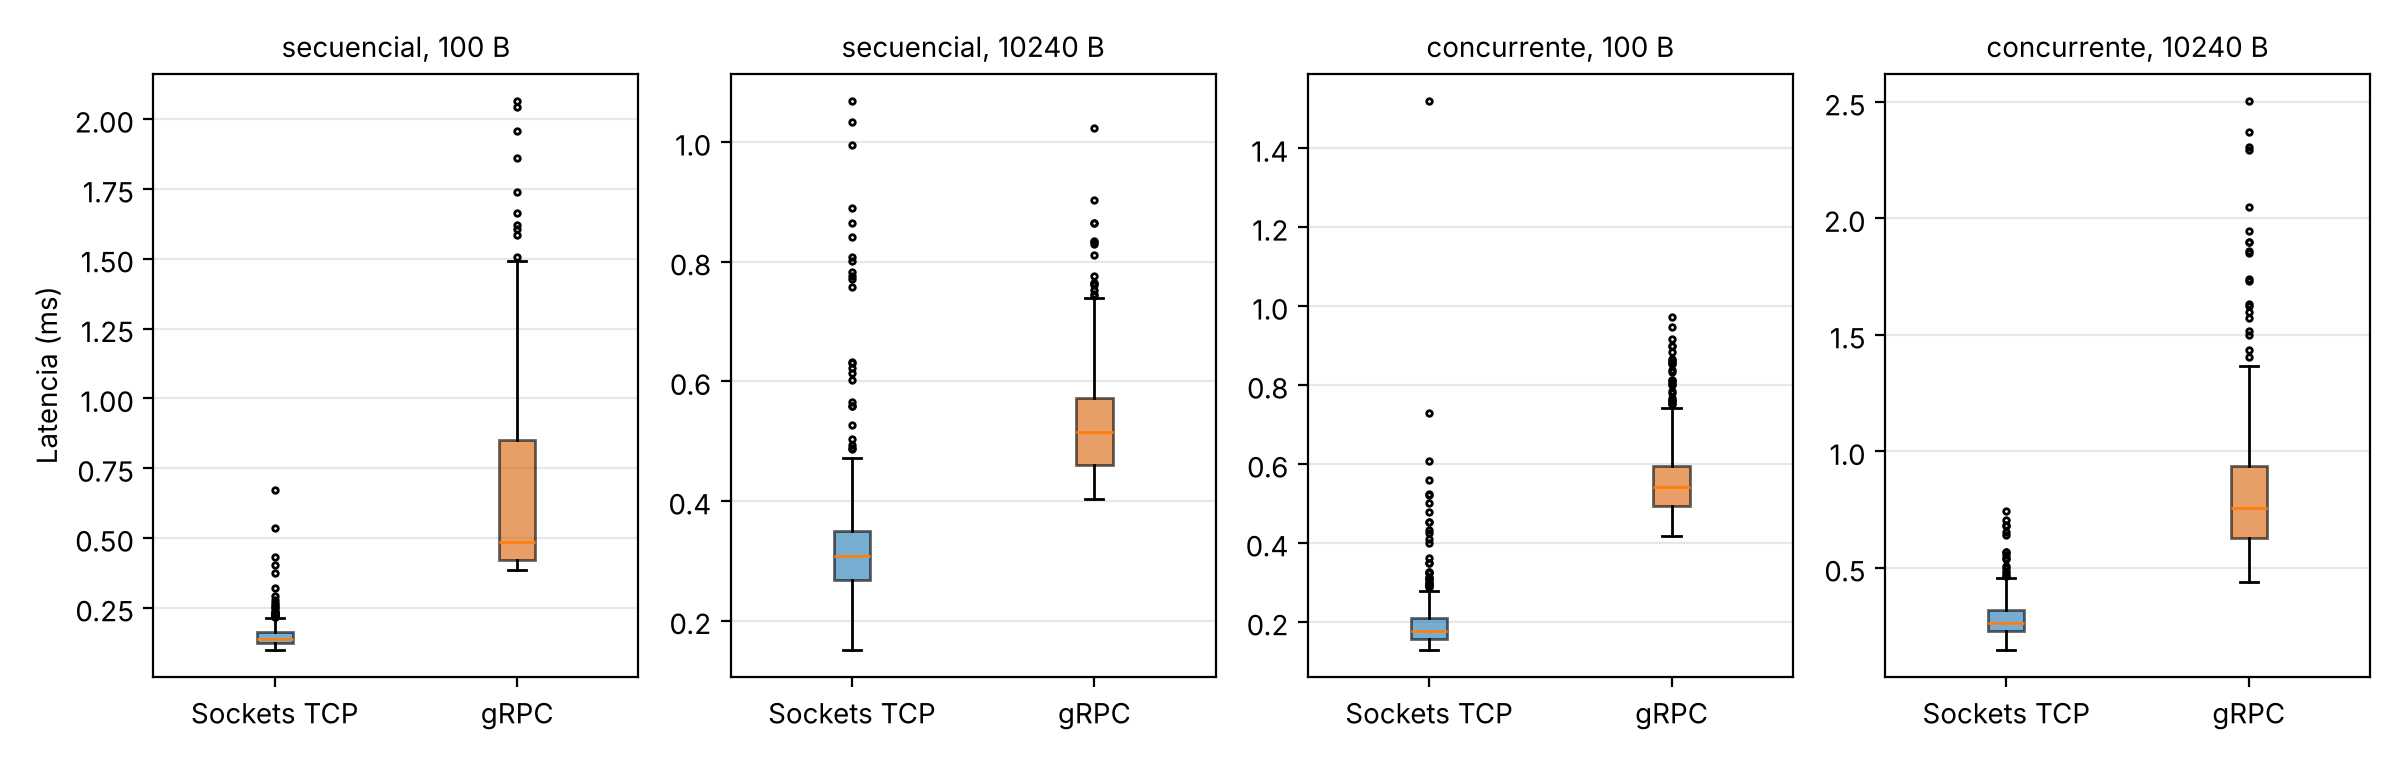
\includegraphics[width=\linewidth]{../resultados/graficos/latencia-cajas.png}
\caption{Distribución de la latencia por mecanismo, tamaño y modo.}
\label{fig:latencia-cajas}
\end{figure}

\begin{figure}[htbp]
\centering
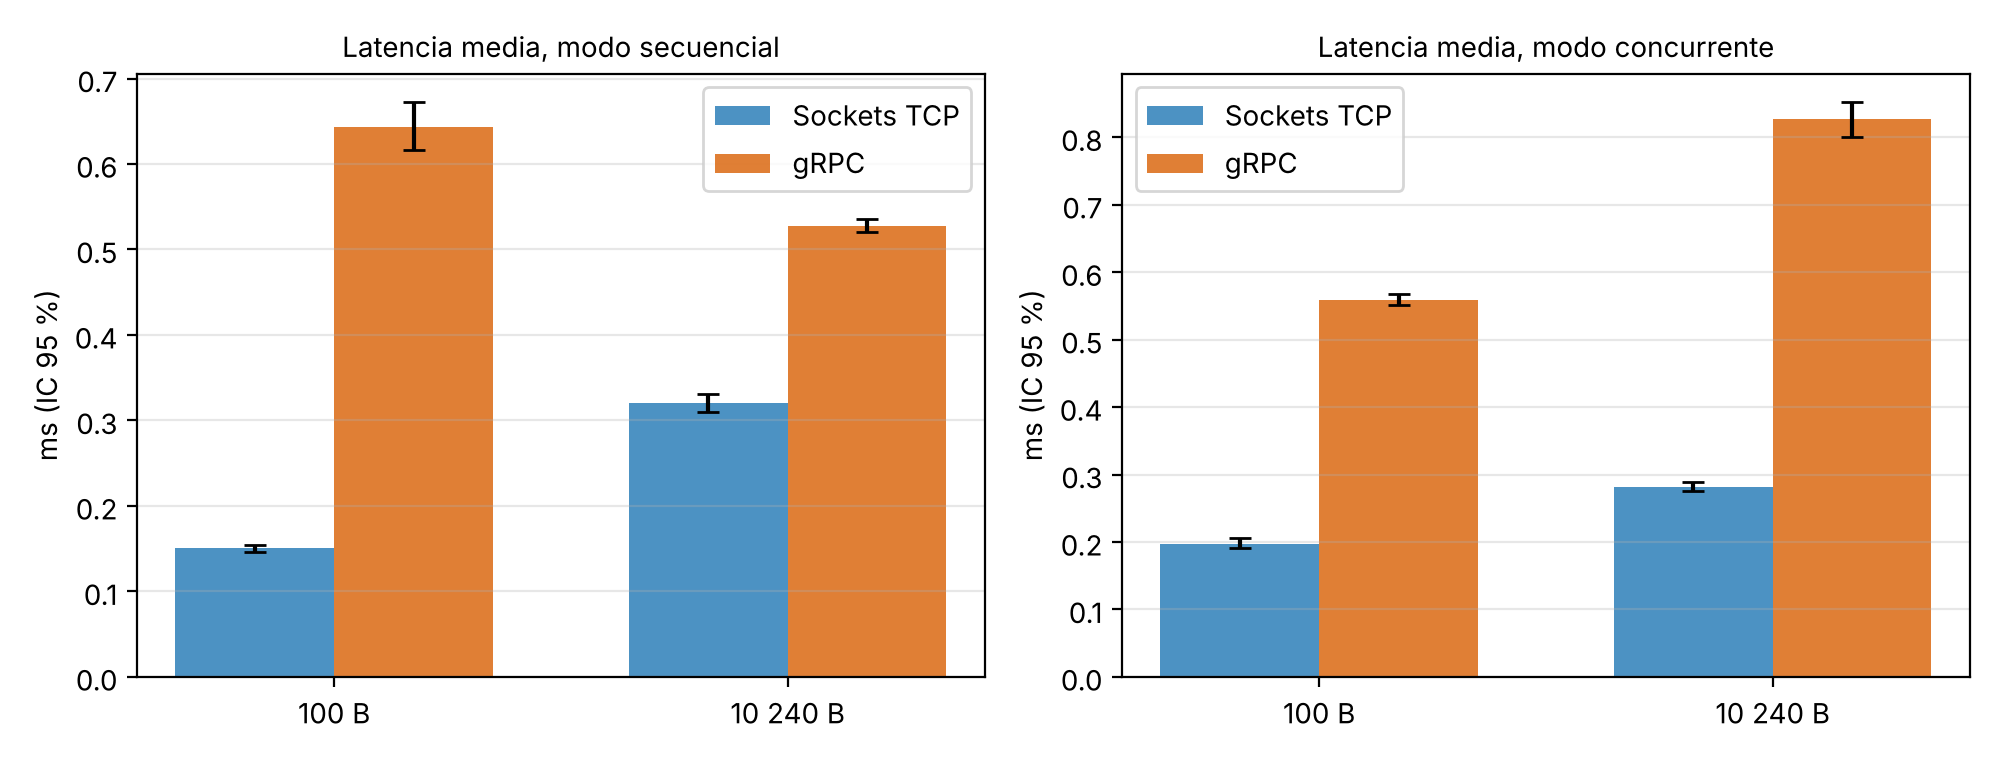
\includegraphics[width=\linewidth]{../resultados/graficos/latencia-media-ic95.png}
\caption{Latencia media con intervalo de confianza del 95\,\%.}
\label{fig:latencia-media}
\end{figure}

\begin{figure}[htbp]
\centering
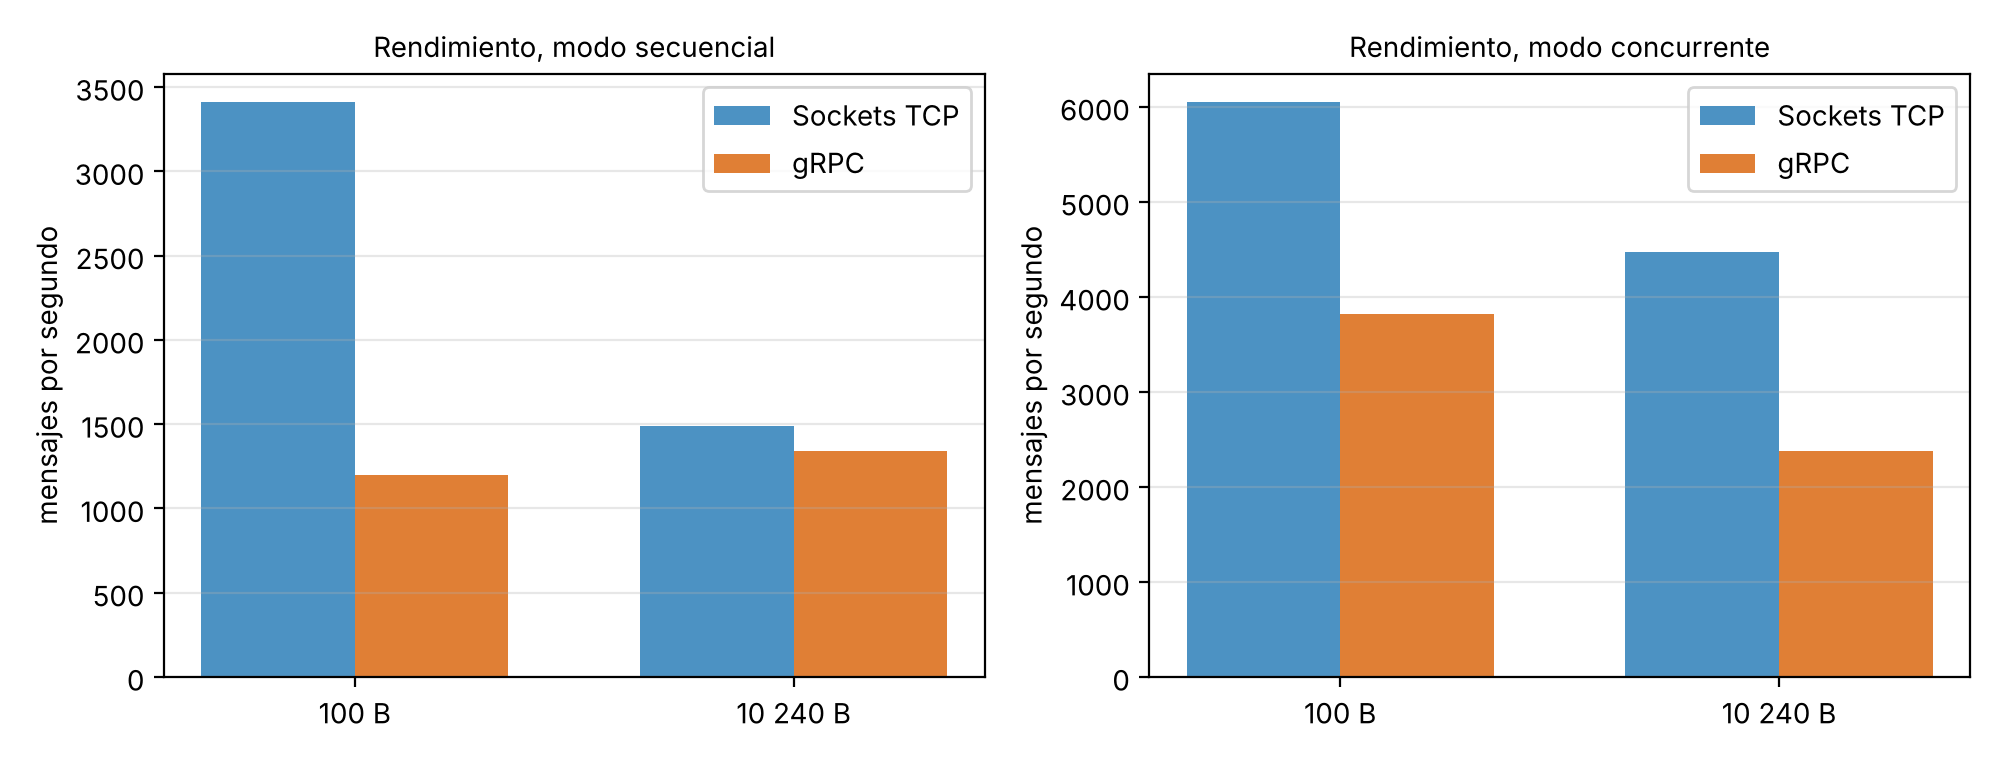
\includegraphics[width=\linewidth]{../resultados/graficos/rendimiento.png}
\caption{Rendimiento en mensajes por segundo.}
\label{fig:rendimiento}
\end{figure}

En las cuatro combinaciones de tamaño y modo, los sockets TCP tuvieron menor latencia media y mayor rendimiento que gRPC, y los intervalos de confianza de las medias no se superponen. La diferencia es mayor con mensajes de 100 bytes en modo secuencial, donde la media de gRPC (0,644\,ms) es unas 4,3 veces la de los sockets (0,150\,ms). Con 10\,240 bytes en modo secuencial la brecha se reduce: 0,528\,ms frente a 0,320\,ms, unas 1,65 veces. En modo concurrente la relación es de unas 2,8 veces con 100 bytes y 2,9 con 10\,240 bytes.

El rendimiento sigue el mismo orden. En modo secuencial, los sockets alcanzaron 3\,409 mensajes por segundo con 100 bytes y 1\,486 con 10\,240, frente a 1\,199 y 1\,342 de gRPC. En modo concurrente fueron 6\,047 y 4\,469 contra 3\,814 y 2\,373.

Hay un dato que conviene leer con cuidado: la media de gRPC con 100 bytes en modo secuencial (0,644\,ms) es mayor que con 10\,240 bytes (0,528\,ms), pero la mediana es menor (0,484 frente a 0,515\,ms). La desviación estándar de esa combinación es la más alta (0,311\,ms) y su p95 es 1,206\,ms, así que la media está arrastrada por envíos lentos aislados, como muestra la Figura~\ref{fig:latencia-cajas}. Con las medianas el orden entre ambos tamaños es el esperado.

\subsection{Verificación del reloj de Lamport}

El script \path|analysis/verificar_lamport.py| se ejecutó sobre los CSV de eventos de los tres nodos de cada mecanismo: la corrida de 20 solicitudes (80 eventos y 40 mensajes emparejados, contando solicitudes y acuses) y la corrida de empate (8 eventos y 4 mensajes). En las cuatro ejecuciones se cumplieron las tres comprobaciones: todo mensaje tiene su envío y su recepción, el reloj de recepción es mayor que el de envío, y el reloj de cada nodo crece de forma estricta. El informe completo está en \path|resultados/lamport.txt|.

En la corrida de empate, tanto en sockets como en gRPC, los envíos \texttt{E-A} (nodo-A) y \texttt{E-B} (nodo-B) tienen reloj 1 y ninguno ocurre antes del otro según los relojes vectoriales calculados a partir de los mismos eventos. Así se observa que el valor de Lamport no basta para ordenar eventos concurrentes: dos eventos con el mismo reloj pueden no estar relacionados causalmente.

\subsection{Limitaciones}

\begin{itemize}
  \item Los tres nodos corren como procesos de un mismo equipo y se comunican por \texttt{localhost}; no hay latencia de red real, por lo que los resultados no se pueden extrapolar a una red distribuida.
  \item Es una sola campaña, con cinco corridas registradas por combinación y un solo equipo. Los intervalos de confianza describen la variación entre envíos de esa campaña, no entre equipos ni días distintos.
  \item Los nodos TCP y gRPC los implementaron personas distintas del equipo; aunque se usó el mismo ejecutor, la misma política de tiempo de espera y las mismas rutas, parte de la diferencia puede deberse a la implementación y no al protocolo. Este análisis no mide la causa de la diferencia.
\end{itemize}
